% Chapter 4

\chapter{HomeLive Management Platform} % Main chapter title

\label{Chapter4} % For referencing the chapter elsewhere, use \ref{Chapter4}

\lhead{Chapter 4. \emph{HomeLive Management Platform}} % This is for the header on each page - perhaps a shortened title

%----------------------------------------------------------------------------------------
In this chapter, the Homelive Management Platform structure will be introduced. The following \autoref{fig:Platform} shows an global view for CWMP. With TR-069 protocol, ACS can communicate and manage devices easily.
%http://orange-france.com.francetelecom.fr:81/ui_normandie/spip.php?article3304
\begin{figure}[htbp]
	\centering
		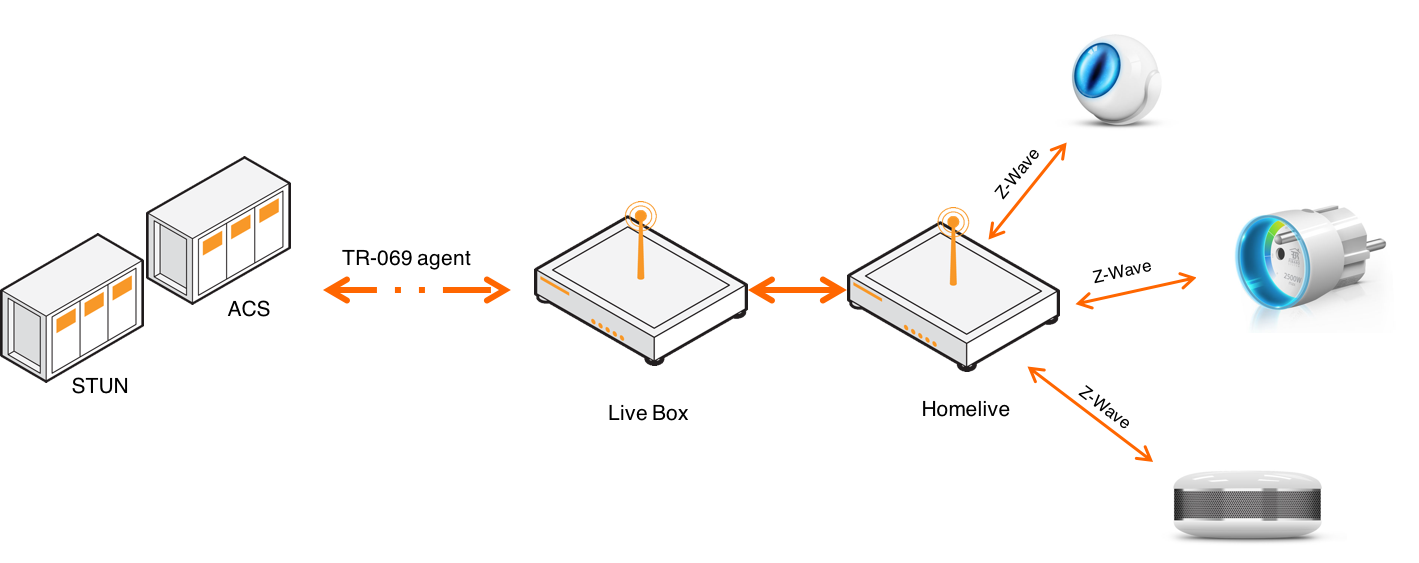
\includegraphics[width=9.5cm]{Figures/Homelive_Management_Platform.png}
	\caption[Homelive Management Platform]{Homelive Management Platform}
	\label{fig:Platform}
\end{figure}

ACS is the server which is accessible by the support engineers of Orange. Support engineers are capable to build a connection remotely with Homelive box using protocol TR-069. The connection are build by two programs. The \textit{TR-069 server} will be running in ACS as a server side and \textit{TR-069 client} will be running in Homelive as the client side. This essentially means that control over the flow of the provisioning session is the sole responsibility of the device. Through TR-069, the high-level operations possible are:
\begin{itemize}
  \item Service activation and reconfiguration
  \begin{itemize}
    \item Initial configuration of the service as part of zero-touch or one-touch configuration process
    \item Service re-establishment (ex. after device is factory-reset, exchanged)
  \end{itemize}
  \item Remote Subscriber Support
  \begin{itemize}
    \item Verification of the device status and functionality
    \item Manual reconfiguration
  \end{itemize}
  \item Firmware and Configuration Management
  \begin{itemize}
    \item Firmware upgrade/downgrade
    \item Configuration backup/restore
  \end{itemize}
  \item Diagnostics and monitoring
  \begin{itemize}
    \item Throughput (TR-143) and connectivity diagnostics
    \item Parameter value retrieval
    \item Log file retrieval
  \end{itemize}
\end{itemize}
%----------------------------------------------------------------------------------------------------------------------
\section{Auto Configuration Server}
The ACS of Orange BU\footnote{Business Unit} and France is named Karma\footnote{Karma is an ancient Indian word means action, work, ordeed. It also refers to the spiritual principle of cause and effect.}, the objective is to manage the Orange devices which are deploied in clients' home.

It is consisted by two PFS\footnote{PlateForm of Service}, one for the TV ecosystem( name Karma STB, only for France), the other one called Historique which is for Orange Livebox on France and for Orange Spain. The server are situated at:
\begin{itemize}
	\item \textbf{Karma LB} situated at the IAC Lyon,
	\item \textbf{Karma STB} situated at the IAC Lille.
\end{itemize}

Karma provides the means to optimise Livebox or Homelive Box upgrades by targeting identified population groups, such as the customers of a new package, for example. Migrations are a more manageable size and conducted as and when. To make best use of the data held in the upgrade platform, Karma is interfaced with applications in the order-delivery process and after-sales service. This inventory function, Papyrus, provides support agents with valuable information on customers’ software upgrades and Voice over IP activation (hardware type, software version, user behaviour through the number of boots, etc.). Karma is based on international standards so that it can be used by all the Group’s business units.

\section{Client-Premise Equipment}
On the client side of TR-069 is the CPE,which is Livebox and Homelive in our case. The Livebox is connected to Internet and serves as a gateway device, it is responsible to provide the connection between TR-069 server and client. Homelive box is the CPE in the strcture, the process view is as \autoref{fig:process}

\begin{figure}[htbp]
	\centering
		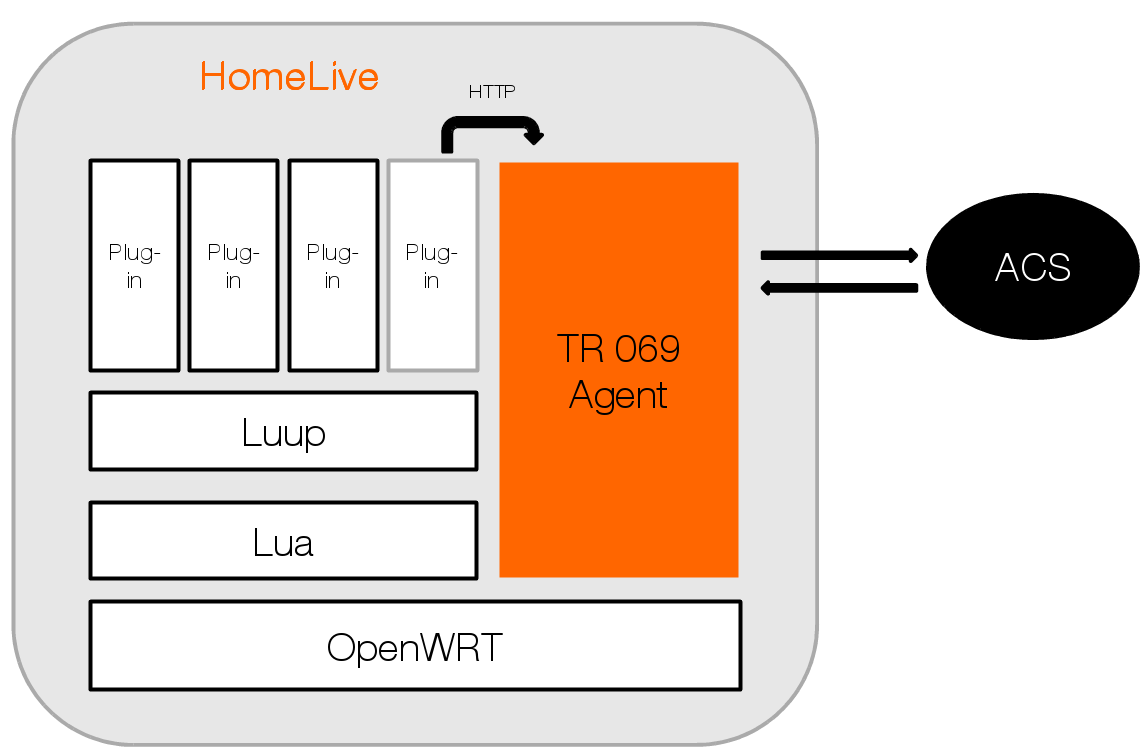
\includegraphics[width=9.5cm]{Figures/process.png}
	\caption[Homelive Process Structure]{Homelive Process Structure}
	\label{fig:process}
\end{figure}

The OpenWRT is the operating system at the base, and beyond is Luup based on Lua. The Luup also provides us the way to create the plug-in, on which we can develop the API satisfying our personnal needs. An API handle the http request is already integrated in the Luup to which we can push the HTTP Request to retrieve the Mios Data Model. Besides that is our TR-069 Client process, the TR-069 Client process will push the request at every starting of the TR-069 session in order to synchronize the Mios Data Model and Z-Wave Data Model.
